\section{Análise e discussão de dados}\label{sec-analiseediss}

Nos experimentos 1, 2 e 3 os grupos de alunos foram expostos,
respectivamente, ao ambiente imersivo em 360º ao ambiente de leitura com
glossário multimodal e ao ambiente imersivo em 360º + ambiente de
leitura com glossário multimodal. A seguir, esses experimentos serão
melhor discutidos.

\subsection{Experimento 1}\label{sub-sec-experimento1}

Neste experimento, 27 alunos foram expostos ao ambiente imersivo em
360º. Primeiramente, eles utilizaram os \emph{desktops} da escola para
explorar livremente o ambiente. Posteriormente, eles fizeram um
\emph{tour} guiado pela pesquisadora pelas cenas do ambiente, durante o
qual a pesquisadora narrou, interativamente, a peça shakespeariana,
fazendo perguntas aos alunos e direcionando sua atenção para objetos nas
cenas. Tais objetos são relevantes tanto para a história, por se
relacionarem a aspectos centrais da trama, quanto para o experimento,
por serem palavras alvo da atividade de aquisição lexical. Essa narração
interativa foi usada tanto para guiar a exploração dos alunos quanto
para ajudá-los a focar sua atenção nos objetos presentes no
ambiente/palavras alvo do experimento. Destaca-se que as palavras alvo
apareceram no ambiente na modalidade visual, sem apoio do verbal.

Simultaneamente à exploração guiada, os alunos responderam às perguntas
de compreensão, outra forma de salientar as palavras alvo e
apresentá-las aos alunos na modalidade escrita. Assim, cada item lexical
foi apresentado repetidas vezes e através de três modalidades
diferentes: visual, sonora e verbal. Esse reforço dos estímulos é
relevante, pois, como apontam pesquisas na área, apresentar o estímulo
em diferentes modalidades contribui significativamente para o
aprendizado e retenção do vocabulário da LE \cite{chun1996,saito2015,procopio2016,mayer2001,monteiro2021}.

Os resultados obtidos por meio dos testes de vocabulário aplicados aos
alunos antes e após a exposição ao ambiente são evidenciados no \Cref{graph-01}.

\begin{figure}[htpb]
    \centering
    \begin{minipage}{.75\textwidth}
    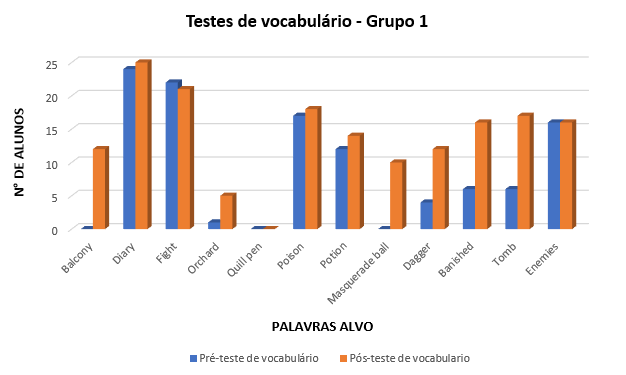
\includegraphics[width=\textwidth]{graph-01.png}
    \caption{Resultado dos Testes de vocabulário do Grupo 1}.
    \label{graph-01}
    \source{Elaborado pelas autoras (2024).}
    \end{minipage}
\end{figure}

Detalhando o gráfico, com base nos dados coletados, percebe-se que o
grupo de alunos exposto ao ambiente de aprendizagem imersivo em 360º
mostrou um ganho de aprendizagem para a maioria das palavras testadas.
Observa-se, entretanto, que algumas palavras tiveram ganho mais
expressivo de aprendizagem após a exposição ao ambiente, como
\emph{balcony, masquerade ball, dagger, banished} e \emph{tomb}
(respectivamente, 44\%, 37\%, 29\%, 37\% e 40\%), enquanto outras
apresentaram um ganho menos expressivo, como \emph{diary, poison} e
\emph{potion} (respectivamente, 4\%, 4\% e 7\%), ou nenhum ganho de
aprendizagem (\emph{fight}, \emph{quill pen} e \emph{enemies}). Essa
diferença pode ser atribuída à importância de cada palavra na narrativa,
pois, apesar de todas serem palavras-chave da tragédia, as que
apresentaram maior ganho de aprendizagem se relacionam diretamente aos
momentos de maior destaque/tensão da narrativa, a exemplo da famosa cena
de Romeo e Julieta na sacada (\emph{balcony}) e do final trágico do
casal na tumba (\emph{tomb}) da família Capuleto.

Conjectura-se que o relativamente baixo ganho de aprendizagem deste
grupo se deve à ausência do verbal (palavra escrita) no ambiente, visto
que apenas a narração não é suficiente para que alunos de nível
elementar consigam inferir o significado das palavras a partir do
contexto e relacioná-las aos objetos presentes no ambiente. Ademais, a
atividade de compreensão realizada durante a exploração do ambiente
também não foi eficaz devido à falta de simultaneidade na apresentação
das modalidades verbal e visual, o que contradiz o Princípio da
Contiguidade \cite{mayer2002} para a elaboração de materiais multimodais.
Segundo este princípio há uma aprendizagem mais profunda quando palavras
e imagens são apresentadas simultaneamente.

Quanto à análise qualitativa, o questionário deste grupo contou com 10
assertivas que visavam avaliar a experiência dos alunos com a atividade,
considerando fatores como usabilidade, engajamento, motivação, atenção e
aprendizagem multimodal. As respostas obtidas podem ser observadas no
\Cref{graph-02}.

\begin{figure}[htpb]
    \centering
    \begin{minipage}{.75\textwidth}
    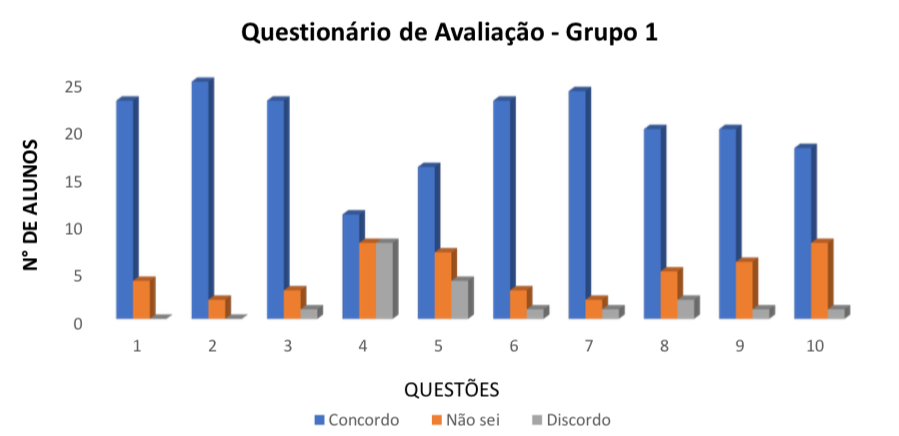
\includegraphics[width=\textwidth]{graph-02.png}
    \caption{Questionário de avaliação da experiência do grupo 1.}
    \label{graph-02}
    \source{Elaborado pelas autoras (2024).}
    \end{minipage}
\end{figure}

A partir das assertivas 1 e 2 (``Usar e interagir com o ambiente foi
fácil para mim'' e ``Aprendi a usar o ambiente de forma rápida e
fácil'') comprova-se a usabilidade do ambiente, visto que 85\% e 92\%
dos alunos, respectivamente, concordaram com elas. Quanto à
aceitabilidade, 85\% concordaram com a assertiva 3 (``A experiência de
aprender vocabulário com ambiente imersivo foi gratificante para mim'').
Quanto ao envolvimento, 41\% afirmaram sentir-se envolvidos durante a
aprendizagem lexical no ambiente, concordando com a assertiva 4 (``Eu me
senti tão envolvido aprendendo vocabulário com o ambiente imersivo que
ignorei tudo ao meu redor''). Esses resultados evidenciam que o ambiente
é fácil e intuitivo de usar, além de favorecer ao engajamento dos alunos
nas atividades. Ele contribui também na criação de um espaço mais
receptivo e motivador para o aprendiz.

As assertivas 5 e 6 averiguaram o direcionamento do foco atencional
proporcionado pelo ambiente. 59\% dos alunos concordaram, 26\% não
souberam responder e 15\% discordaram da assertiva 5 (``O ambiente
ajudou a focar minha atenção nas informações relevantes para a
aprendizagem do vocabulário''). Isso aponta para o potencial do ambiente
enquanto recurso pedagógico, pois ajuda a direcionar a atenção dos
alunos ao objeto de aprendizagem, condição necessária para a ocorrência
do \emph{noticing} (registro cognitivo) e, consequentemente, do
aprendizado \cite{schmidit1990}. Ainda, através da assertiva 6 (``A narração
da professora durante a exploração do ambiente me ajudou a focar a
atenção nos objetos relacionados ao vocabulário''), verificou-se a
pertinência da narração durante o \emph{tour} guiado enquanto estratégia
essencial para ajudar os participantes a focarem sua atenção no objeto
de aprendizagem, como afirmaram 85\% dos alunos.

As assertivas 7 e 8 (``Eu gostei de estudar/aprender vocabulário com
esse ambiente'' e ``Eu me senti mais motivado aprendendo vocabulário com
esse ambiente que com materiais mais tradicionais (ex. livro
didático)''), comprovam a satisfação dos alunos com a aprendizagem
lexical mediada pelo ambiente. Os dados mostram 88\% dos alunos
afirmaram ter gostado de aprender vocabulário através do ambiente e 74\%
concordaram que ele motiva mais que materiais didáticos tradicionais.
Conjectura-se que a multimodalidade presente no ambiente, através da
interatividade e da novidade, é responsável por fazer com que os alunos
se sintam mais motivados em realizar as atividades e, assim, aprender a
LE.

As assertivas 9 e 10 (``Esse ambiente me permitiu compreender melhor o
significado das palavras, podendo ver objetos e relacioná-los à
história'' e ``O ambiente imersivo e os recursos utilizados durante sua
exploração foram suficientes para que eu aprendesse o vocabulário'')
corroboram a efetividade da aprendizagem multimodal, pois 74\% dos
alunos concordaram com a assertiva 9 e 67\%, com a 10, o que ratifica o
papel da multimodalidade como facilitadora do processo de ensino e
aprendizagem, pois a apresentação do material por meio de diferentes
modalidades facilita a compreensão do vocabulário alvo \cite{mayer2001}.

\subsection{Experimento 2}\label{sub-sec-experimento2}

Neste experimento, 27 alunos foram expostos ao ambiente de leitura com
glossário multimodal. Eles ficaram livres para explorá-lo, podendo ler
informações essenciais dos personagens principais e o hipertexto da peça
teatral Romeo e Julieta, cujos \emph{links} (palavras-alvo do
experimento) lhes direcionavam ao glossário multimodal, onde podiam ver
a representação em 2D, a pronúncia e o significado das palavras-alvo.
Não foi feita nenhuma intervenção durante a exploração desse ambiente,
deixando os alunos totalmente livres para navegá-lo e aprender o
vocabulário da forma como preferissem. Os resultados obtidos nos testes
de vocabulário deste experimento podem ser vistos no \Cref{graph-03}.

\begin{figure}[htpb]
    \centering
    \begin{minipage}{.75\textwidth}
    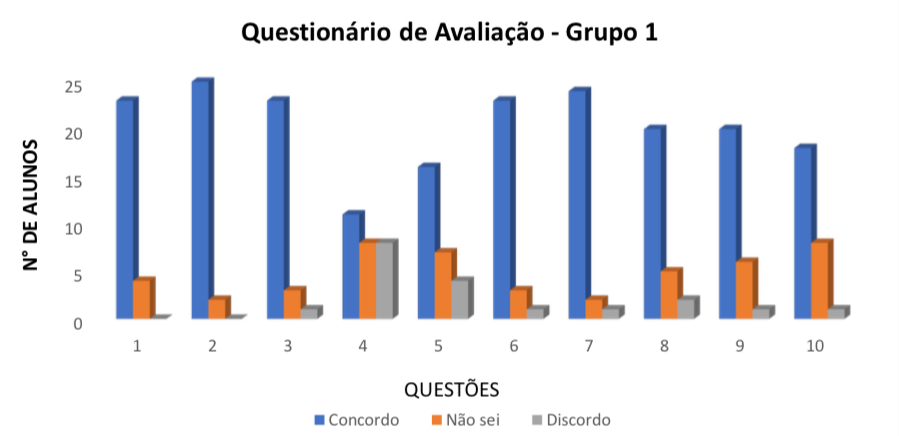
\includegraphics[width=\textwidth]{graph-03.png}
    \caption{Resultado dos Testes de vocabulário do Grupo 2.}
    \label{graph-03}
    \source{Elaborado pelas autoras (2024).}
    \end{minipage}
\end{figure}

Semelhantemente ao experimento 1, o grupo de alunos expostos ao ambiente
de leitura com glossário multimodal também mostrou ganho de aprendizagem
para quase todas as palavras, com exceção de \emph{fight,} e
\emph{enemies}, cujo conhecimento dos alunos antes e após a exposição se
manteve o mesmo. Contudo, percebe-se que, no geral, o ganho de
aprendizagem por palavra foi mais expressivo neste grupo. Por exemplo,
as palavras \emph{quill pen, masquerade ball} e \emph{tomb} apresentaram
um ganho de, respectivamente, 52\%, 52\% e 67\% no experimento 2, mas de
0\%, 38\% e 38\% no grupo 1. Pode-se atribuir essa diferença à presença
da multimodalidade neste ambiente, que se mostra mais eficaz para a
aprendizagem de alunos de proficiência elementar. Isso ocorre porque
este ambiente oferece o apoio do hipertexto e do glossário multimodal,
possibilitando a visualização da forma escrita das palavras-alvo, de seu
significado e imagens correspondentes. Assim, destaca-se a relevância da
apresentação simultânea de palavras escritas e imagem para a
aprendizagem de vocabulário \cite{mayer2001}, visto que as modalidades
verbal e visual são apresentadas aos alunos de forma simultânea.

Já questionário de avaliação da experiência deste grupo possuía 11
assertivas e foi adaptado para contemplar as características do ambiente
de leitura, mas o objetivo foi o mesmo: avaliar a experiência dos
alunos, considerando fatores como usabilidade, engajamento, motivação e
atenção para responder à segunda pergunta desta pesquisa. Os resultados
obtidos podem ser verificados no \Cref{graph-04}.

\begin{figure}[htpb]
    \centering
    \begin{minipage}{.75\textwidth}
    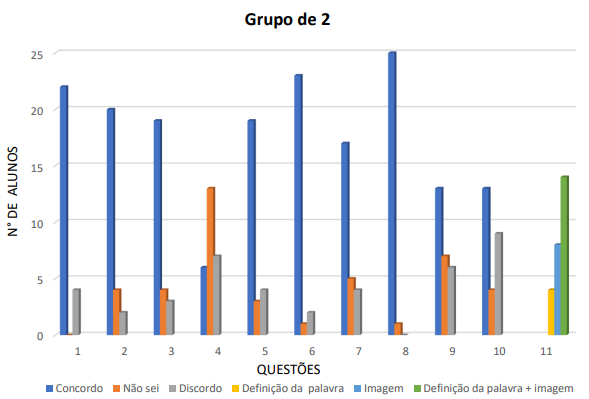
\includegraphics[width=\textwidth]{graph-04.png}
    \caption{Questionário de avaliação da experiência Grupo 2.}
    \label{graph-04}
    \source{Elaborado pelas autoras (2024).}
    \end{minipage}
\end{figure}

Percebe-se que fator usabilidade deste ambiente foi corroborado pelos
alunos, pois 81\% concordaram com a assertiva 1 (``Usar e interagir com
o ambiente foi fácil para mim.'') e 74\%, com a assertiva 2 (``Aprendi a
usar o ambiente de forma rápida e fácil.''). Em relação à
aceitabilidade, 70\% concordaram que a experiência de aprender
vocabulário com o ambiente foi gratificante, fator averiguado através da
assertiva 3 (``A experiência de aprender vocabulário com o glossário
multimodal foi muito gratificante para mim.''). Quanto ao envolvimento
com o ambiente, 22\% concordaram, 52\% não souberam responder e 26\%
discordaram da assertiva 4 (``Eu me senti tão envolvido aprendendo
vocabulário com o glossário multimodal que ignorei tudo ao meu redor).

Quanto à atenção focada, 70\% concordaram com a assertiva 5 (``O
ambiente de leitura com glossário multimodal ajudou a focar minha
atenção nas informações relevantes para a aprendizagem do
vocabulário.''). Assim, evidencia-se que o ambiente ajuda o aluno a
direcionar sua atenção ao objeto de aprendizagem, o que, segundo a
\emph{Noticing Hypothesis} \cite{schmidit1990}, é necessário para ocorrer o
\emph{noticing}. Logo, o ambiente se mostra um recurso pedagógico de
relevância, pois ajuda a promover o registro cognitivo das informações,
promovendo a aprendizagem.

Ademais, 85\% concordaram com a assertiva 6 (``Eu gostei de
estudar/aprender vocabulário com o glossário multimodal.''). Isso aponta
para a agradabilidade proporcionada pelo ambiente \cite{schumann1999neurobiology}, a
qual está relacionada a fatores emocionais ligados à aprendizagem da LE,
como a motivação. Essa foi melhor averiguada através da assertiva 7
(``Eu me senti mais motivado estudando vocabulário com o glossário
multimodal que com materiais tradicionais (ex.: livro didático)''), com
a qual 63\% dos alunos concordaram, 22\% não souberam responder e 15\%
discordaram. Isso mostra que o ambiente possui mais potencial para
motivar os alunos durante a aprendizagem de vocabulário que materiais
didáticos tradicionais/lineares. Atribuímos isso à multimodalidade
presente no ambiente, um recurso que, por meio da interatividade e da
novidade, é capaz de fazer com que os alunos se sintam mais motivados
durante a atividade.

Quanto à aprendizagem multimodal, 92,5\% dos participantes concordaram
com a assertiva 8 (``O glossário me permitiu compreender melhor o
significado das palavras do texto por meio de imagens, pronúncias e
definições.''), evidenciando a eficácia da multimodalidade na
aprendizagem de vocabulário. Isso ocorre, pois a combinação de
diferentes modalidades no glossário permite melhor compreensão das
palavras-alvo, como defende a Teoria Cognitiva de Aprendizagem
Multimídia \cite{mayer2001}. Ademais, 48\% dos alunos concordaram com a
assertiva 9 (``O glossário multimodal foi suficiente para que eu
aprendesse o vocabulário.''), enquanto 30\% não souberam responder e
22\% discordaram. Isso mostra que, embora o glossário multimodal seja
eficaz, a utilização de recursos adicionais pode tornar a aprendizagem
lexical em ambientes multimodais ainda mais eficaz. Logo, surge a
necessidade de testar a eficácia da combinação de outras modalidades
além das utilizadas neste ambiente, o que será averiguado no terceiro
experimento.

Por questões técnicas, não foi possível reproduzir a pronúncia das
palavras presentes no glossário. Por meio da assertiva 10 (``\emph{A
impossibilidade de ouvir a pronúncia das palavras no glossário não
prejudicou minha aprendizagem do vocabulário''}), verificou-se se isso
gerou prejuízos à aprendizagem das palavras. 48\% dos alunos afirmaram
que isso não prejudicou a aprendizagem do vocabulário, enquanto 33\%
discordaram dessa assertiva e 19\% não souberam responder. Porém, o som
é um recurso relevante para os aprendizes de nível elementar e, por
isso, em futuras utilizações deste ambiente de aprendizagem, deve haver
um empenho para que todas as modalidades estejam disponíveis para o
pleno uso dos alunos.

Por fim, na assertiva 11 (``Qual dos recursos presentes no glossário
mais contribuíram para sua aprendizagem do vocabulário?''), buscou-se
averiguar qual das modalidades presentes no glossário foi mais eficaz
para a aprendizagem do vocabulário. Assim, 55,5\% dos alunos apontaram
``palavras + imagem'' como o recurso que mais contribui para sua
aprendizagem no ambiente, enquanto 29,5\% apontaram a ``imagem'' e 15\%,
a ``definição da palavra''. Esse resultado também corrobora a Teoria
Cognitiva de Aprendizagem Multimídia \cite{mayer2001}, a qual defende que
se aprende melhor através de palavras e imagens que apenas de palavras.

\subsection{Experimento 3}\label{sub-sec-experimento3}

No experimento 3, 27 alunos foram expostos ao ambiente de aprendizagem
imersivo em 360º + ambiente de leitura com glossário multimodal.
Primeiramente, eles exploraram o ambiente de leitura, podendo, a
qualquer momento, clicar nos \emph{links} e consultar o significado, a
pronúncia e a representação em 2D das palavras-alvo no glossário
multimodal. Isso pode facilitar a compreensão do significado dessas
palavras e constitui outra forma de salientá-las para além das
repetições no texto, pois a saliência é um fator importante para a
retenção lexical na memória a longo prazo \cite{procopio2016,saito2015}.

Após essa livre exploração do ambiente de leitura, os participantes
foram direcionados para o ambiente imersivo em 360º, no qual fizeram um
\emph{tour} pelas cenas do ambiente guiados pela pesquisadora, que
retomou oralmente o enredo de Romeu e Julieta, salientando as
palavras-alvo e direcionando a atenção dos participantes para os objetos
em 360º, também palavras-alvo do experimento. Essa estratégia teve o
intuito de salientar os objetos, pois a plataforma não permite a
inserção das palavras-alvo na modalidade escrita e o destaque desses
objetos para ficarem mais salientes para os alunos. Os resultados
obtidos neste experimento podem ser vistos no \Cref{graph-05}.

\begin{figure}[htpb]
    \centering
    \begin{minipage}{.75\textwidth}
    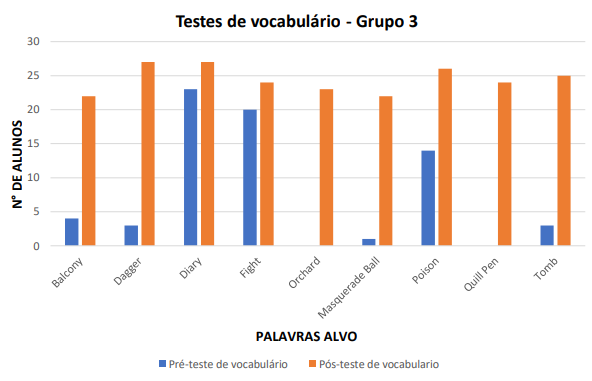
\includegraphics[width=\textwidth]{graph-05.png}
    \caption{Resultado dos Testes de vocabulário do Grupo 3.}
    \label{graph-05}
    \source{Elaborado pelas autoras (2024).}
    \end{minipage}
\end{figure}

Com base nos resultados dos testes de vocabulário dos alunos expostos à
terceira condição de testagem, observa-se um ganho de aprendizagem mais
expressivo para a maioria das palavras em comparação aos dois grupos
anteriores, com destaque para as palavras \emph{dagger, orchard},
\emph{masquerade ball} e \emph{quill pen}, com ganhos de,
respectivamente, 100\%, 73\%, 66\%, 68\% e 63\%.

Esses resultados nos levam a acreditar que, quando os ambientes são integrados,
a aprendizagem lexical é potencializada. Isso se deve aos diferentes recursos
presentes em cada um deles, que, combinados, fazem com que mais modalidades
estejam disponíveis. Isso é corroborado por \textcite{lemke2002}, o qual
postula que o significado das diferentes modalidades é multiplicativo, fazendo
do todo mais que a simples soma das partes e contribuindo, assim, para a
realização de inferências e retenção do significado inferido na memória.
Destaca-se também o fator saliência, essencial para a retenção lexical
\cite{procopio2016,saito2015}, pois o grupo 3 foi exposto a cada uma das
palavras-alvo no mínimo três vezes por meio das modalidades verbal, escrita e
visual.

Quanto à análise qualitativa, devido uma greve docente ocorrida durante
a coleta de dados deste estudo, no início ano de 2024, e à consequente
paralização das atividades do colégio de aplicação em que o experimento
foi aplicado, o questionário de avaliação da experiência deste grupo
precisou ser reduzido e, por isso, diferiu-se dos aplicados aos grupos
anteriores, enfocando mais diretamente a atenção, a motivação e a
aprendizagem multimodal. Através da primeira pergunta discursiva (Você
gostou da atividade? Justifique sua resposta.), averiguou-se que o
ambiente promove a agradabilidade, pois todos os participantes afirmaram
ter gostado da atividade. Segundo \cite{schumann1999neurobiology}, a agradabilidade
promove motivação e engajamento do aluno, facilitando o processo de
aprendizagem. Logo, conclui-se que o ambiente é capaz de promover a
motivação nos alunos durante a aprendizagem de vocabulário.

Na segunda pergunta (Você acha que a atividade te ajudou a aprender
vocabulário?), buscou-se averiguar se a aprendizagem mediada pelo
ambiente é eficaz para a aquisição lexical. Semelhantemente à pergunta
anterior, todos os alunos afirmaram que a atividade ajudou na sua
aprendizagem de vocabulário. Vê-se que o ambiente é capaz de auxiliar os
alunos a direcionarem sua atenção ao objeto de aprendizagem durante a
realização da atividade, promovendo o aprendizado. Isso corrobora a
\emph{Noticing Hypothsis} \cite{schmidit1990}, segundo a qual, para que o
aprendizado ocorra, o aluno deve direcionar sua atenção para o objeto de
aprendizagem para registrá-lo cognitivamente (\emph{noticing}) e
aprendê-lo. Assim, conclui-se que, sem atenção, não há aprendizagem.
Logo, o ambiente, capaz de atrair e direcionar a atenção dos alunos,
mostra-se um recurso pedagógico eficiente para a aprendizagem de LE.

Na terceira pergunta (Qual dos itens abaixo mais contribuiu para o seu
aprendizado de vocabulário durante a atividade?), buscou-se averiguar
qual dos recursos utilizados no ambiente mais contribuiu para a
aprendizagem do vocabulário em LE: a narração do texto; o glossário; a
peça teatral ``Romeu e Julieta''; ou a exploração do ambiente guiada
pela pesquisadora. A opção a mais escolhida foi a exploração guiada do
ambiente (54\%), seguida pelo glossário (27\%), narração (13\%) e peça
teatral (6\%). Logo, conclui-se que o tour guiado pela pesquisadora,
além de suprir limitações do ambiente, mostrou-se um recurso muito
eficaz para a aprendizagem do vocabulário, pois orientou a exploração do
ambiente e direcionou a atenção dos alunos, possibilitando a ocorrência
do \emph{noticing} (registro cognitivo), condição necessária para que o
aprendizado ocorra \cite{schmidit1990}. Além disso, aponta-se a eficácia do
glossário multimodal enquanto recurso que auxilia a aquisição lexical
mediada por ambientes multimodais, pois, além de fornecer um suporte
escrito aos alunos, facilita a aprendizagem ao apresentar o vocabulário
através de diferentes modalidades, o que corrobora a Teoria Cognitiva de
Aprendizagem Multimídia \cite{mayer2001}, pois o uso de duas ou mais
modalidades possibilita que o aluno construa representações mentais mais
ricas e estabeleça relação entre elas, facilitando a aprendizagem.
